%Chapter 3

\renewcommand{\thechapter}{3}
\newcommand{\KrCal}{$\rm^{83m}Kr \: $}
\newcommand{\Rb}{$\rm^{83}Rb \: $}

\chapter{Corrections to the S1 and S2 signals}
\label{Ch:3}

In this chapter we address the spatially-dependent corrections applied to the S1 and S2 signals. During the 2013 science run, \KrCal injections were performed periodically to measure the position-dependent corrections. The better we can correct the S1 and S2 signals for position-dependance, the smaller the signal variations will be, leading to better background rejection for the WIMP search. 


%After the energy deposit occurs in the active region of the LUX detector the freed electrons are drifted via electric field towards the liquid surface. The S2 light is emitted as the electrons are extracted at a given x,y position from the liquid surface and accelerated by a 6 kV potential, traversing 5mm from the liquid surface to the anode. 
The dominant correction is typically made on the S2 signal, considering the free electron lifetime. As charge drifts from the event site to the extraction region (0-47 cm), it may become attached to electronegative impurities in the liquid. S2s of equal sizes are exponentially attenuated with increasing drift distance in the detector by impurities such as $\rm O_2$, $\rm H_2O$, $\rm N_2$ (3 ppb $\rm O_2$ corresponds to roughly 100 $\rm \mu s$ lifetime \cite{GPM}). The S2 signal also has x and y variations due to non-uniformities in the extraction field, tilt in the liquid level, and non-uniformities in the anode-gate separation. 


Unlike the charge signal, the S1 light propagates isotropically from the interaction site and has about a 30\% variation in light collection efficiency between events near the top and bottom of the detector due to geometric effects. For events in the  bulk liquid xenon, about 2/3 of the S1 light is collected on the bottom PMT arrays due to total internal reflection at the liquid gas interface. The closer the event to the bottom PMTs, the larger the solid angle of the bottom PMT array, increasing the probability of the detecting a photon and producing a photo electron (PE). Other position-dependent effects include the photon absorption length, which is negligible at the purities achieved in LUX, and teflon reflectivity which is $>$ 90\% in liquid xenon \cite{Teflon_R_1} \cite{Teflon_R_2}. The S1 position-dependent correction used in the LUX analysis normalizes the photon detection probability of all events to the center of the active region, an arbitrary choice corresponding roughly to the average light response.

It should also be noted that variation in light yield and charge yield due to the non-uniformity of the electric field are also folded into x,y,z correction.  The field increases from about 140 to 200 V/cm from the cathode to gate in the LUX detector, the electric field model is shown in \ref{Ch:2}. The effect of light yield and charge yield for \KrCal due to dependance of recombination on the local electric field is on the order of 10\% \cite{NEST_2013}. Also, all S1 and S2 signals are measured as photo electrons (PE) that have been calibrated by pulsing LEDs (450 ns) located inside the TPC. Any quantum efficiency (QE) or gain variations in the 122 PMTs which are not properly normalized by the individual gain corrections are also folded into the position-dependent corrections measured from the $\rm^{83m}Kr$ calibrations.


\section{$\rm^{83m}Kr$ Calibration}

Throughout the science run, periodic $\rm^{83m}Kr$ injections were performed to calculate position-dependent corrections. $\rm ^{83m}Kr$ is produced from the $\rm \beta$ decay $\rm^{83}Rb$ with a half life of 86.2 days. The $\rm^{83}Rb$ source is housed in charcoal and plumbed directly into the LUX circulation system. The decay scheme of \Rb and \KrCal is shown in figure \ref{fig:Kr_Decay}.

\begin{figure}[h!]\centering
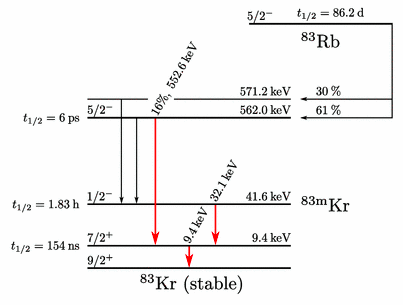
\includegraphics[width=90mm]{Chapter_XYZ_Corr/Thesis_Corr_Plots/RbKr_83_Decay.png}
\caption{A simplified decay diagram of \Rb and \KrCal, from \cite{Kr_Decay_Diagram}.}
\label{fig:Kr_Decay}
\end{figure}

\noindent \KrCal which is continuously produced in the charcoal housing, is a meta-stable excited state of $\rm^{83}Kr$. It has a half-life 1.8 hours. $\rm^{83m}Kr$ decays via an electron capture first emitting a 32.1 keV $\rm \beta$ followed by a 9.4 keV $\rm \beta$ with a half life of 154 ns for the intermediate state \cite{Start_Kr} \cite{Kastens}.  For the vast majority of the decays, LUX observes the combined S1 pulse corresponding to 41.55 keV, since the minimum S1 pulse separation in the LUX reconstruction is 1000 ns. Figure \ref{fig:Kr_Waveform} (a) and (b) shows two \KrCal events with the decay of the 32.1 and 9.4 keV $\rm \beta$ separated by 60 and 220 ns, respectively. The two S1s are classified as a single S1 event by LUX in both cases. The timing separation between the S1 and S2 is used to infer the drift distance to be 14.0 and 40.0 cm below the liquid surface, respectively. The attenuation of the S2 signal due to electronegative impurities is apparent by comparing the amplitudes of the S2 signals, with roughly 50\% charge loss. The S2 pulses are insensitive to the timing separation of the dual decay as electron diffusion smears the charge deposits together as the electrons drift through the active region before extraction \cite{Electron_Diffusion}. The PMT hit map for the events is shown in figure \ref{fig:Kr_Hit_Map}.


\renewcommand{\baselinestretch}{1}
\small\normalsize
\begin{figure}[p!]\centering
 
\subcaptionbox{\KrCal event with 60 ns timing separation. \label{fig:Kr_a}}{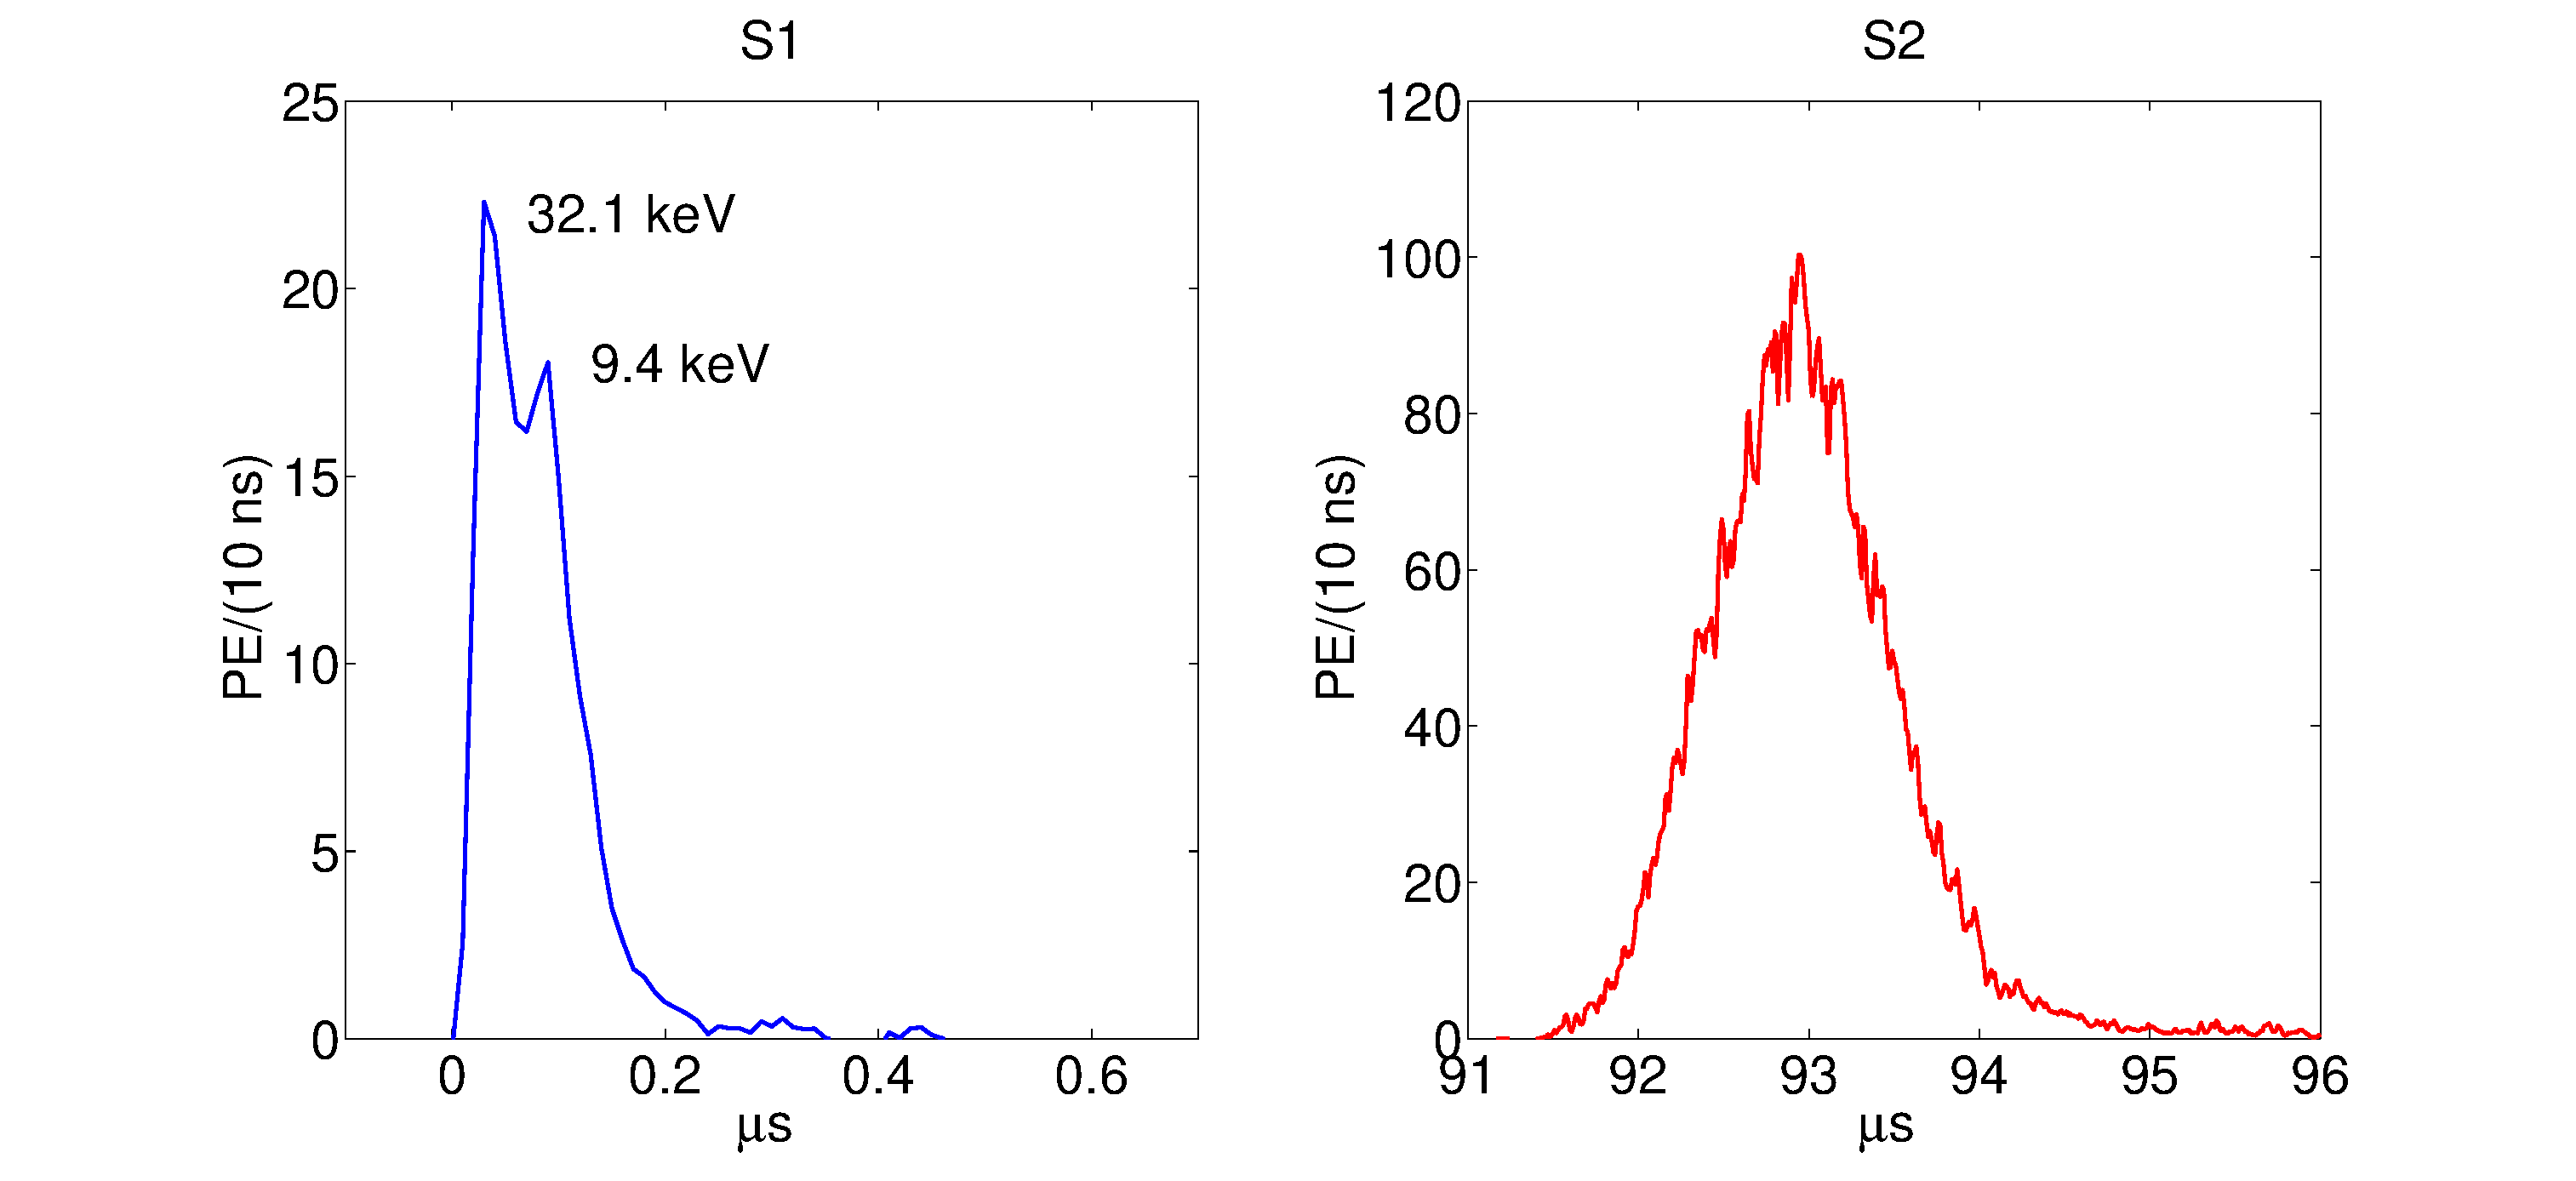
\includegraphics[width=130mm]{Chapter_XYZ_Corr/Thesis_Corr_Plots/Kr_Merged_Waveform.eps}}
\subcaptionbox{\KrCal event with 220 ns timing separation.\label{fig:Kr_b}}{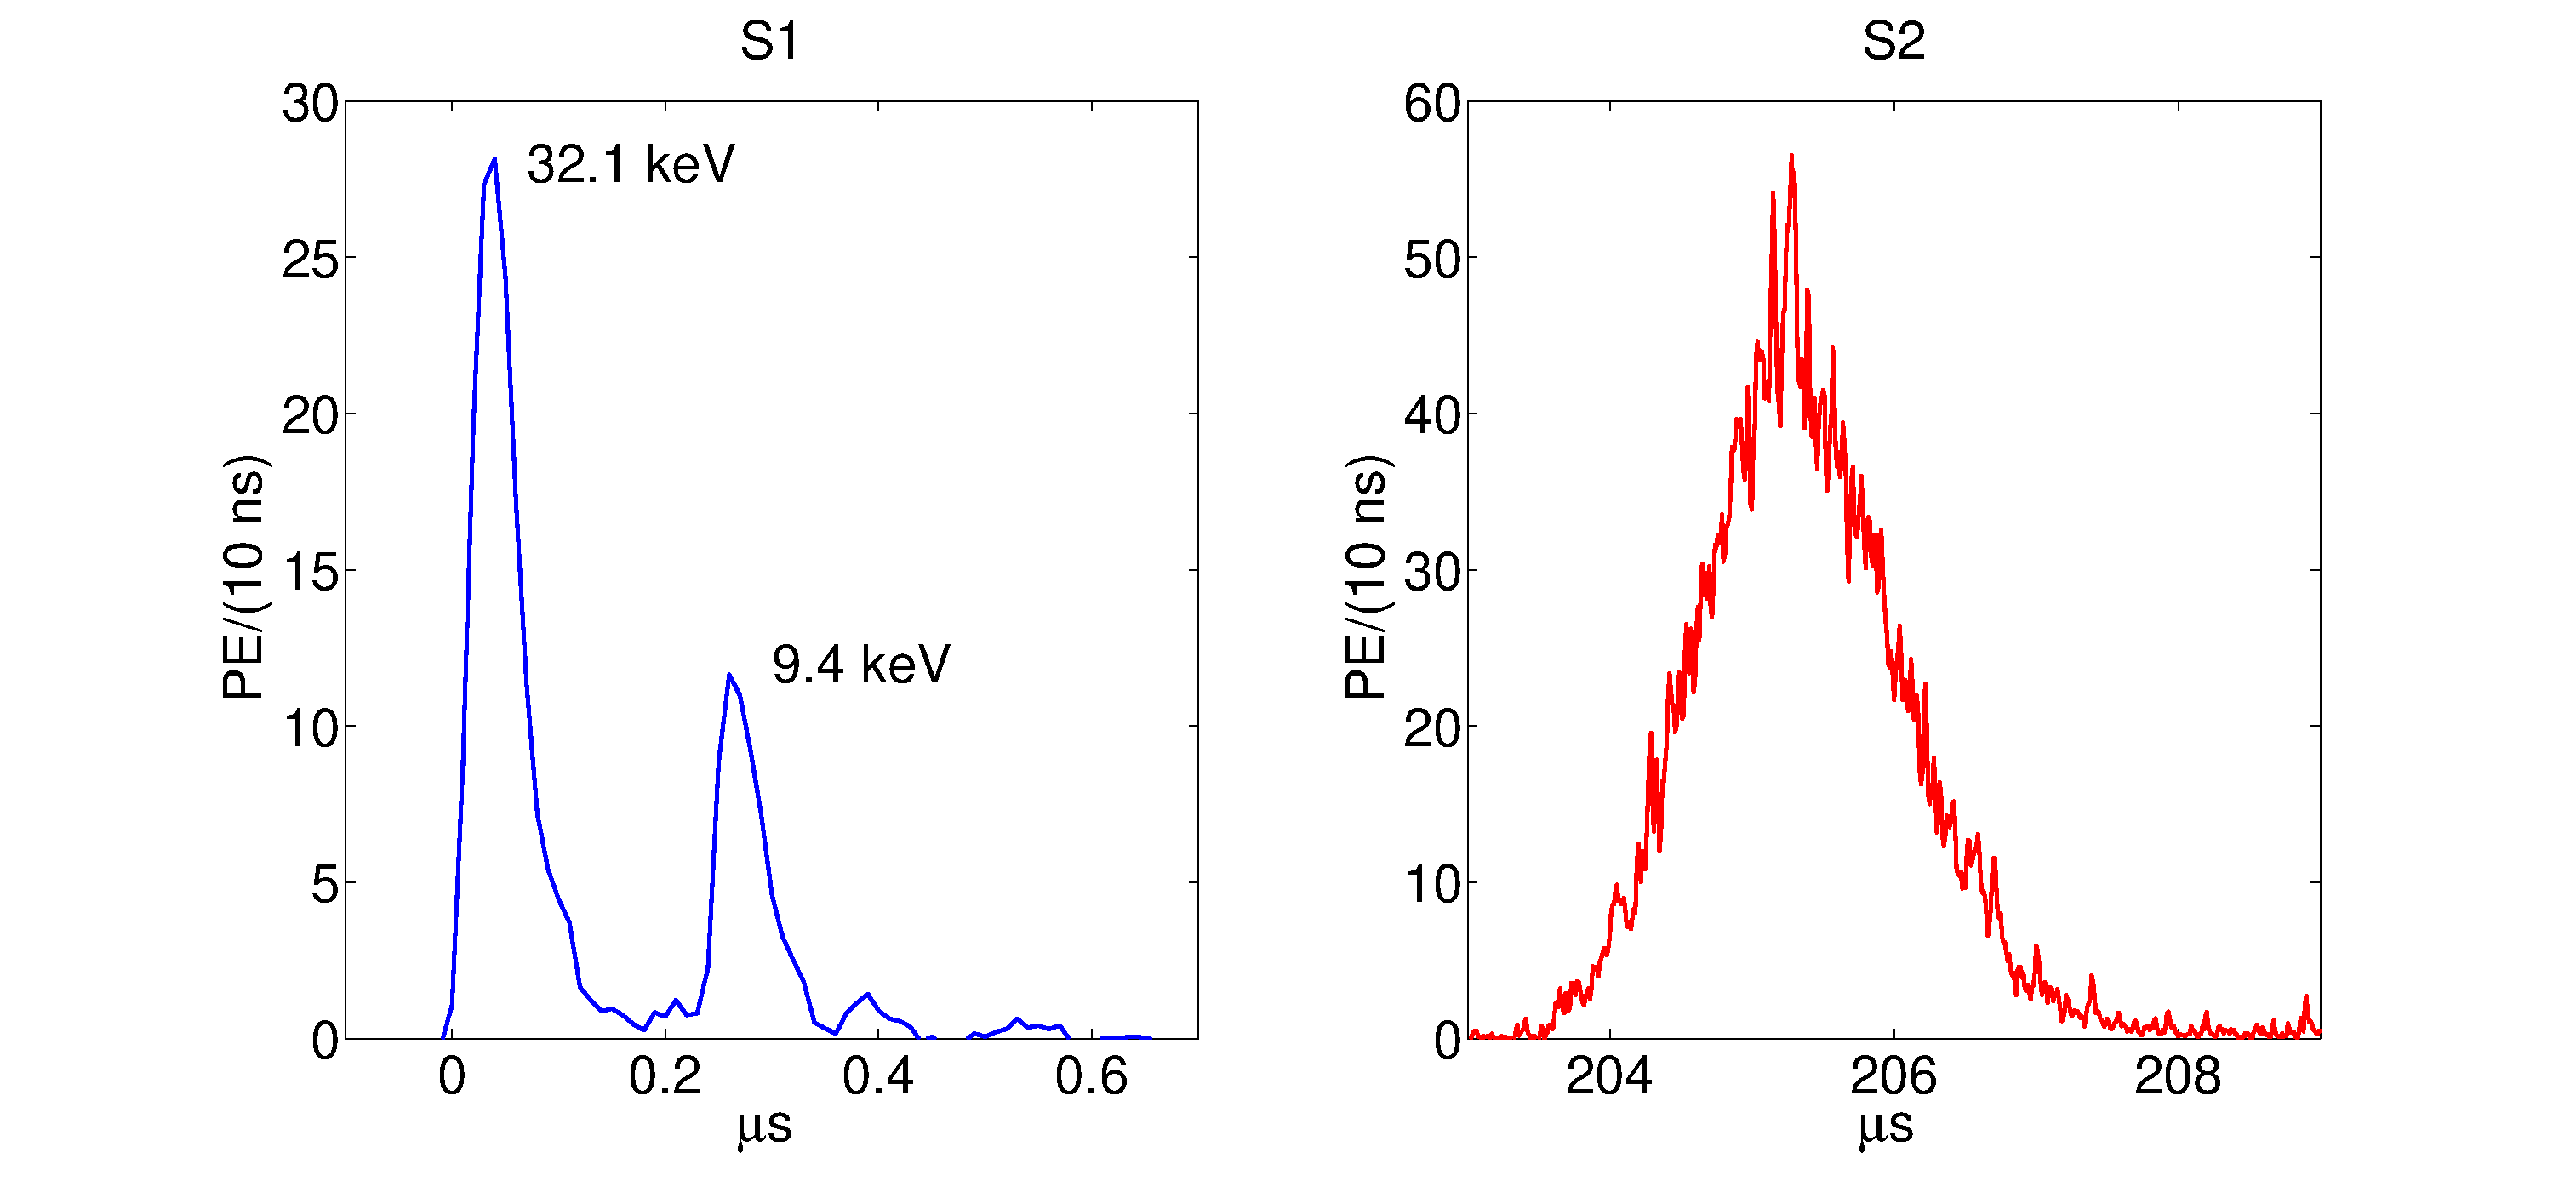
\includegraphics[width=130mm]{Chapter_XYZ_Corr/Thesis_Corr_Plots/Kr_Split_Waveform.eps}}

\caption{The S1 and S2 of two \KrCal events. (a): A \KrCal event in which the two decays have overlapped within 60 ns. The S2 arrives about 93 $\rm \mu s$ later. Bottom Figures (b): A \KrCal event in which the two decays have overlapped within 220 ns. The S2 arrives about 205 $\rm \mu s$ later. The LUX pulse finder classifies events within a 1$\rm \, \mu s$ window as a single S1. The S2 pulses are insensitive to the timing separation of the dual decay as electron diffusion smears the pulses two together as the electrons drift. The PMT hit map for these events are shown below in figure \ref{fig:Kr_Hit_Map}.}
\label{fig:Kr_Waveform}
\end{figure}
\renewcommand{\baselinestretch}{2}
\small\normalsize


\renewcommand{\baselinestretch}{1}
\small\normalsize
\begin{figure}[h!]\centering
 
\subcaptionbox{\KrCal event with 60 ns timing separation. \label{fig:Kr_a}}{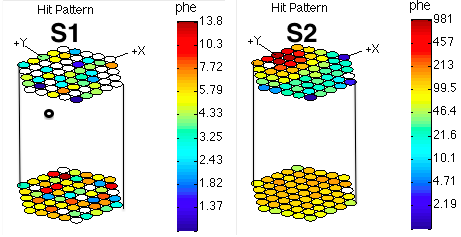
\includegraphics[width=130mm]{Chapter_XYZ_Corr/Thesis_Corr_Plots/Kr_Evt_Merged_HitMap.png}}
\subcaptionbox{\KrCal event with 220 ns timing separation.\label{fig:Kr_b}}{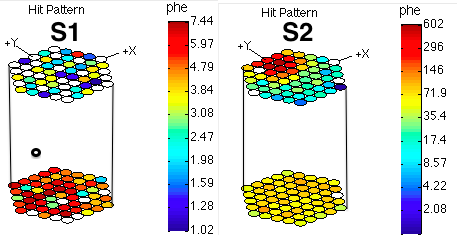
\includegraphics[width=130mm]{Chapter_XYZ_Corr/Thesis_Corr_Plots/Kr_Evt_Split_HitMap.png}}

\caption{The S1 and S2 of two \KrCal events. Top Figures (a): A \KrCal event in which the two decays have overlapped within 60 ns. Bottom Figures (b): A \KrCal event in which the two decays have overlapped within 220 ns. The black, open circle represents the location of the event. The S1 hit pattern is diffuse with more light collected on the bottom arrays due to total internal reflection at the liquid surface. The S2 is localized in the top PMT arrays in x,y at the location where the electrons are extracted, and diffuse on the bottom due to scattering. The summed waveforms for these events are shown in figure \ref{fig:Kr_Waveform}.}
\label{fig:Kr_Hit_Map}
\end{figure}
\renewcommand{\baselinestretch}{2}
\small\normalsize

\newpage

\section{\KrCal Mixing in Liquid Xenon}

\KrCal is introduced when needed into the LUX detector by flushing the charcoal housing with xenon gas and diverting the flow inline with the main circulation path. The \KrCal source and its delivery into the xenon detector is described in more detail in \cite{Kastens}. The relatively short half-life of 1.8 hours allows for several injections per week, as the source decays to negligible levels within hours. Once injected, the activity is uniformly mixed into the liquid xenon within minutes. Figure \ref{fig:Kr_Dist} shows the uniform distribution of \KrCal events in the LUX detector thirty minutes after the injection. Once uniformly mixed, the decay of \KrCal produces a well defined mono-energetic peak in the detector. The S1, S2, and energy spectra are shown in section \ref{sec:E_specs}. Measuring the location of the spectral peak vs. event position allows the detector's spatial response to be monitored over the course of the science run.

\newpage

\begin{figure}[h!]\centering
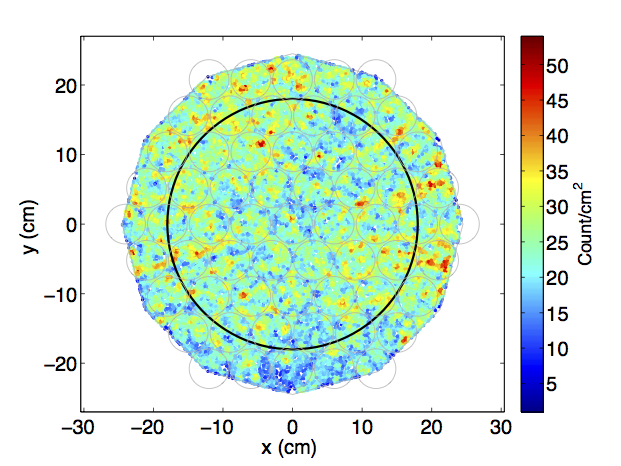
\includegraphics[width=72mm]{Chapter_XYZ_Corr/Thesis_Corr_Plots/Kr_XY_density.png}
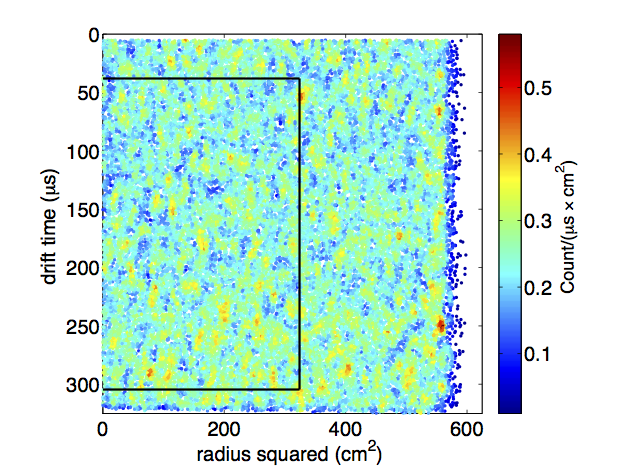
\includegraphics[width=72mm]{Chapter_XYZ_Corr/Thesis_Corr_Plots/Kr_RZ_density.png}
\caption{Distribution of \KrCal events 10 minutes after the injection. The source mixes uniformly throughout the liquid xenon illuminating all regions of the active volume. The solid black lines represent the fiducial volume used for the WIMP search. }
\label{fig:Kr_Dist}
\end{figure}

%uniform illumination.... show decay constant.

\section{S2 Electron Lifetime and x,y Correction}

As mentioned previously, events in LUX have well-defined x,y,z positions computed from the S2 hit pattern (x,y) and the S1-S2 signal separation time (z). The electron lifetime is calculated by binning the detector in drift time into 60 slices. In each slice a Gaussian is fit to to the \KrCal S2 signal to determine the mean. An exponential is fit to the mean S2 response as a function of z, shown in figure \ref{fig:S2_EL}. The characteristic attenuation length is $\lambda = \tau v_{drift}$, where $v_{drift}$ is the electron drift velocity and $\rm \tau$ is the electron lifetime from the exponential fit. For this analysis we use the S2 response of the bottom PMT array ($\rm S2_b$) as it was used for the 2013 WIMP search analysis discussed in Chapter \ref{Ch:2}. %Corrections for top only, bottom only, and all PMTs are computed for each \KrCal calibration data set.


\renewcommand{\baselinestretch}{1}
\small\normalsize
\begin{figure}[h!]\centering
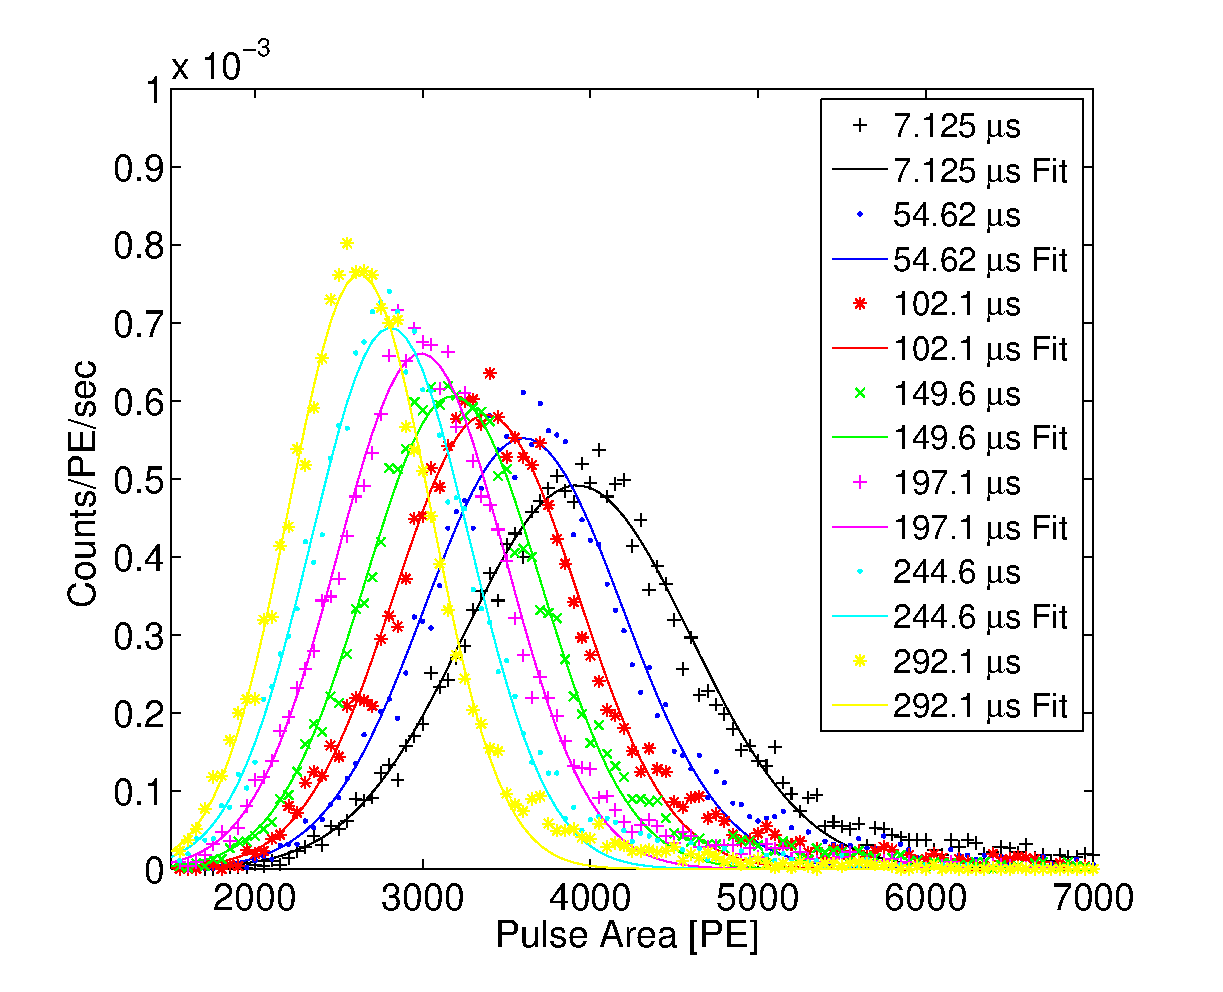
\includegraphics[width=75mm]{Chapter_XYZ_Corr/Thesis_Corr_Plots/S2_bottom_hist_EL.eps}
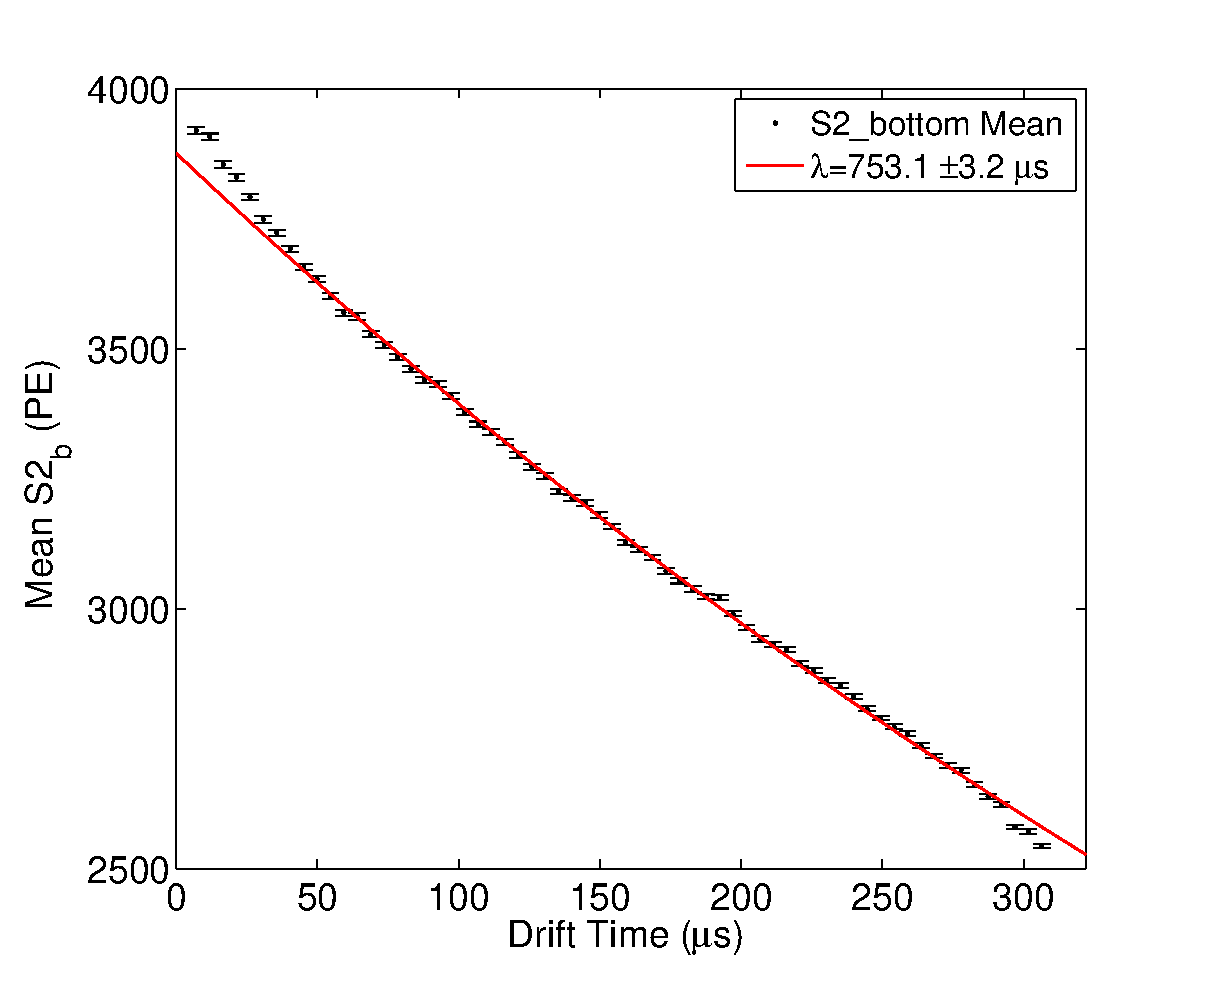
\includegraphics[width=73mm]{Chapter_XYZ_Corr/Thesis_Corr_Plots/S2_bottom_lifetime.eps}
\caption{Left: Fits to the mean of $\rm S2_b$ of the \KrCal data in several z slices. Right, the exponential fit to the means of $\rm S2_b$ vs. drift time used to extract electron lifetime $\rm \tau$. The electron lifetime is found to be $\rm \tau$ = 753.1 $\pm$ 3.2 $\rm \mu s$. The exponential fit to the means deviates near the top and bottom of the active region since the charge yield from the \KrCal decay is sensitive the the varying electric field. The data shown was taken data on May 10, 2013 (lux10\_20130510\_T1250) and contains 700,000 \KrCal events. }
\label{fig:S2_EL}
\end{figure}
\renewcommand{\baselinestretch}{2}
\small\normalsize

To remove the effect of the finite electron lifetime, the z-corrected $\rm S2_b$ from each signal is calculated as follows:
\begin{equation}
\rm S2_{\operatorname{b-z}}=S2_b\cdot exp\left(\frac{drift\,time[\mu s]}{\tau[\mu s]}\right)
\label{eq:S2_Z}
\end{equation}

\noindent Where $\rm S2_{\operatorname{b-z}}$ is the z corrected $\rm S2_b$ signal and $\rm \tau$ is the free electron lifetime. After correcting the dominant z dependent electron attenuation, corrected to 0 drift time, we calculate the normalization factor ($\mathcal{NF}$) that will be used to correct for the x,y dependent variations ing the S2 signal.

The normalization is calculated by creating a 25 x 25 grid on the x-y plane, corresponding to 2 cm x 2 cm x,y bins. For each bin the average $\rm S2_b$ light response is determined by fitting a Gaussian. Figure \ref{fig:S2_XY_norm_center} (left) shows the measured $\rm S2_b$ response to 700,000 $\rm^{83m}Kr$ decays normalized to the response at the center, x=y=0. This map represents the inverse of the normalization factor that we call $\rm\mathcal{NF}(x,y)$. $\mathcal{NF}$ is then applied to the $\rm S2_b$ data by using a spline interpolation of the x,y coordinate of each event relative to the bin centers $\rm\mathcal{NF}(x,y)$. Figure \ref{fig:S2_XY_norm_center} (right) shows the $\rm S2_b$ response after correcting the data relative to the center x=y=0 using $\rm\mathcal{NF}(x,y)$. After applying the x,y correction the variation decreases from 10\% to 1\% in the inner 18 cm radius of the detector (the fiducial volume).

%talk about the bins. 25x25 grid, or 50x 50 grid. (with at least 100 events each to define the mean with a Gaussian)

\begin{figure}[h!]\centering
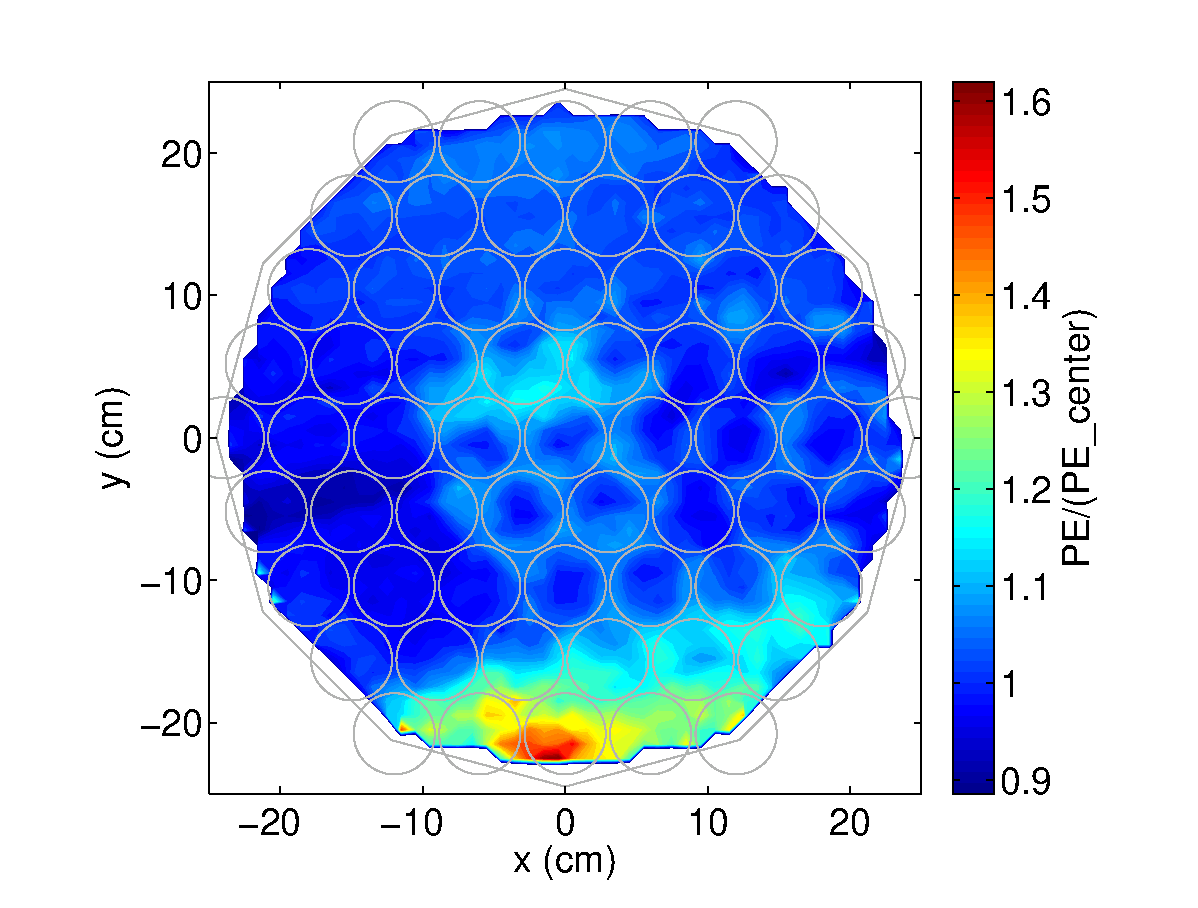
\includegraphics[width=74mm]{Chapter_XYZ_Corr/Thesis_Corr_Plots/S2_b_1cm_1cm/S2_b_XY_1cm_norm.eps}
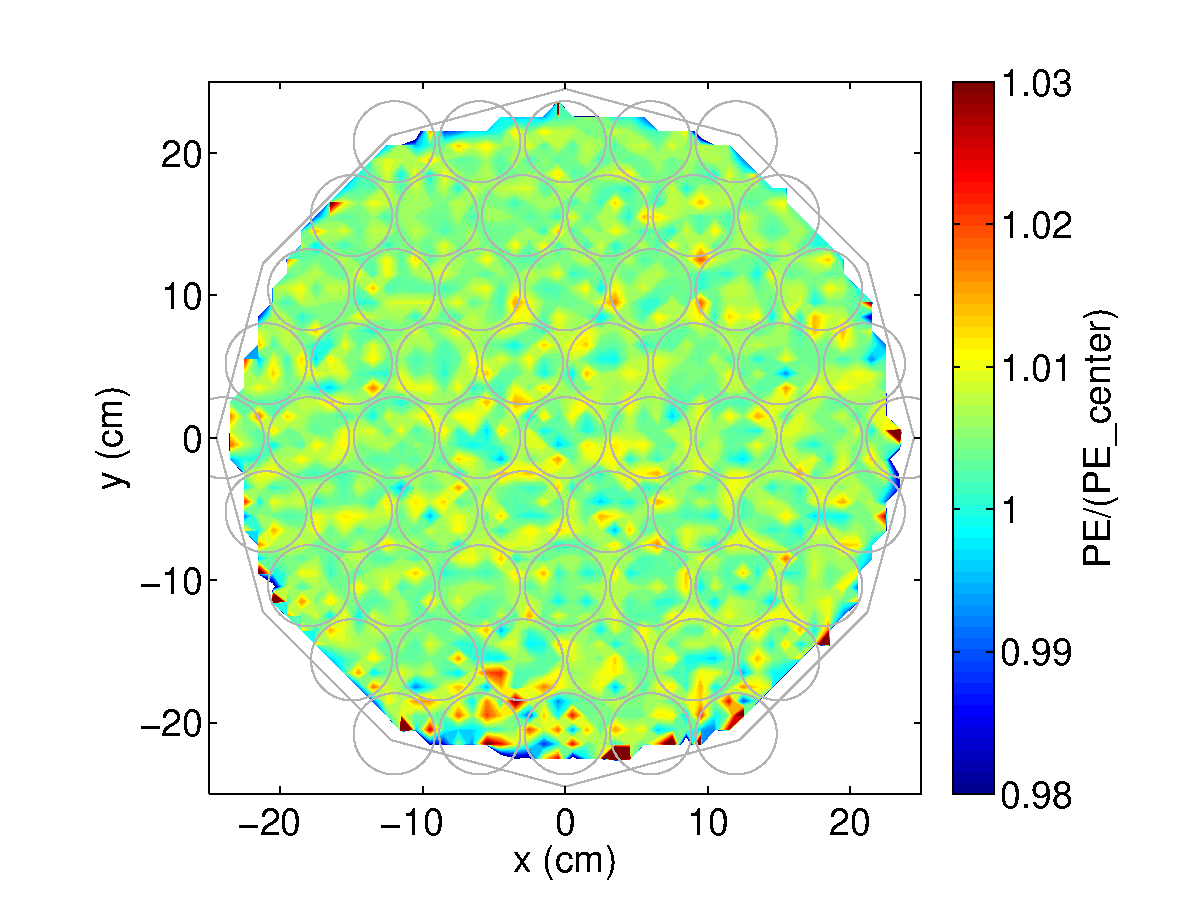
\includegraphics[width=74mm]{Chapter_XYZ_Corr/Thesis_Corr_Plots/S2_b_1cm_1cm/S2_b_XY_1cm_norm_FlatField.eps}
\caption{Left: Response of $\rm S2_b$ vs. x,y normalized to the response at the center (x=y=0). The region of larger response around x=0, y=-25 is likely from an enhanced extraction field between the anode and gate wires. Right: Response of $\rm S2_b$ vs. x,y after correcting the data using $\rm\mathcal{NF}_{S2_b}$. }
\label{fig:S2_XY_norm_center}
\end{figure}


After correcting for z and x,y we can define the position-dependent  (x,y,z) corrected $\rm S2_b$ signal, which we will call $\rm S2{_b}_c$ calculated as follows:
\begin{equation}
\rm S2_{\operatorname{b-c}}=S2_{\operatorname{b-z}} \cdot \mathcal{NF}_{S2_b}(x,y) % removed S2_{\operatorname{b-(x,z,y)}}
\label{eq:S2_XYZ}
\end{equation}

\noindent where $\rm S2_{\operatorname{b-c}}$ is the x,y,z corrected $\rm S2_b$ signal and $\rm \mathcal{NF}_{S2_b}(x,y)$ is the Normalization Factor of the bottom PMT array for S2s and is a function of x,y. The interpolation of the inverse of $\rm \mathcal{NF}_{S2_b}(x,y)$ along the x,y grid is plotted in figure \ref{fig:S2_XY_norm_center}.


Figure \ref{fig:S2_res} shows the improvement in the $\rm S2_b$ signal after applying the z and x,y correction.After applying the z correction to $\rm S2_b$ there is a fractional improvement in resolution of 18\%, for the case of an 750 $\rm \mu s$ electron lifetime. The correcting in the x,y plane provides an additional 4.9\% improvement in resolution to the $\rm S2_b$ signal. 

\renewcommand{\baselinestretch}{1}
\small\normalsize
\begin{figure}[h!]\centering
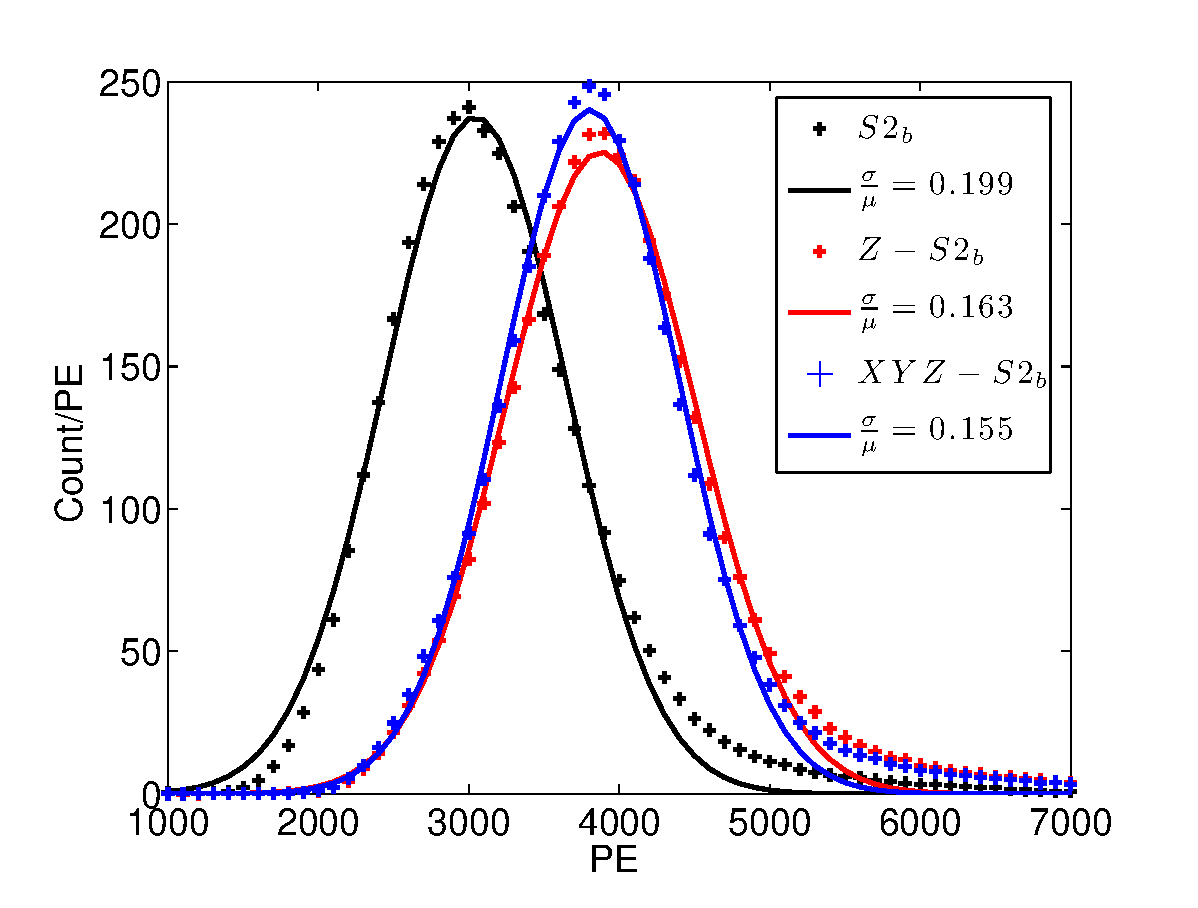
\includegraphics[width=100mm]{Chapter_XYZ_Corr/Thesis_Corr_Plots/S2_corr_res.eps}
\caption{Improvement of resolution in $\rm S2_b$ after applying the z and x,y,z correction. Black: The uncorrected data. Red: The data with only z dependent correction, the electron lifetime correction. Blue: The data with full x,y,z dependent correction. The data shown was taken data on May 10, 2013 (lux10\_20130510\_T1250) and contains 700,000 \KrCal events.}
\label{fig:S2_res}
\end{figure}
\renewcommand{\baselinestretch}{2}
\small\normalsize

\section{S1 x,y,z Correction}

To measure the x,y,z dependent Normalization Factor for S1 ($\rm \mathcal{NF}_{S1}$), we divide the detector into a 25 x 25 x 16 x,y,z mesh with each voxel having dimensions of 2 cm x 2 cm x 20 $\rm \mu s$. To achieve sufficient statistics for the correction we require at least 400,000 $\rm^{83m}Kr$ events, about 40 events per voxel to define the mean. Monthly high stats calibrations are performed that yield about 1 million counts to providing precise $\mathcal{NF}$ correction maps. Unlike the S2 correction, which is highly dependent on purity, the S1 has been found to be invariant to within a percent over the course of the science run, thus the monthly calibrations with high statistics are sufficient to provide the position-dependent correction.

Figure \ref{fig:S1_XYZ_norm_center} shows the response of the detector to $\rm^{83m}Kr$ normalized to the center of the detector in 16 slices of z, each with a 2 cm x 2 cm x,y grid. The plotted maps and normalized to the center of the detector and represent the inverse of the normalization factor ($\rm \mathcal{NF}_{S1}$). We choose to normalize the the center of the detector as it represents the average light collection efficiency of the detector. Though the dominant correction is the z-dependance, there is also substructure in x,y to each z slice which is illustrated in figure \ref{fig:S1_XYZ_norm_center_slice}, where we have normalized each slice to its own center. It is evident that near the top and bottom there are additional geometric effects around the radial edges, whereas in the central z slices the uniformity in x,y is much better due to the diffusion of the light scattering on the teflon.

\renewcommand{\baselinestretch}{1}
\small\normalsize
\begin{sidewaysfigure}[p!]\centering
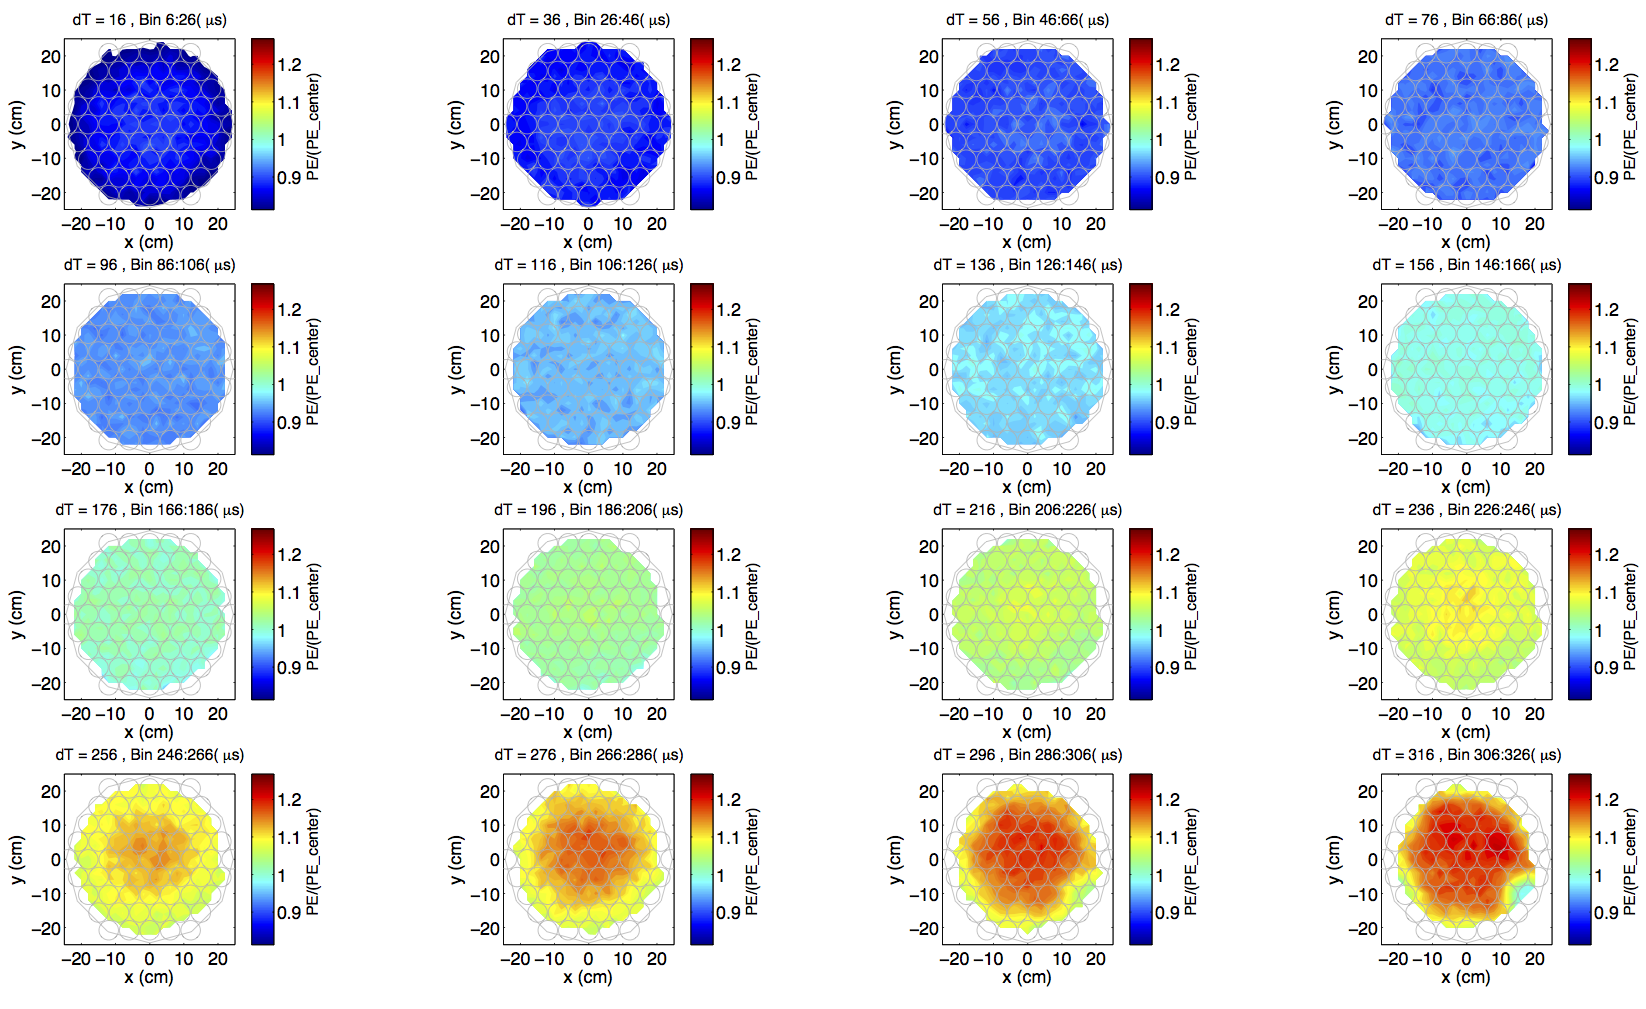
\includegraphics[width=230mm]{Chapter_XYZ_Corr/Thesis_Corr_Plots/S1_XYZ_Kr_norm_center_crop_80.png}
\caption{S1 x,y,z response normalized to the center of the detector. The interpolated map represents the inverse of the normalization factor $\mathcal{NF}$. }
\label{fig:S1_XYZ_norm_center}
\end{sidewaysfigure}
\renewcommand{\baselinestretch}{2}
\small\normalsize

\renewcommand{\baselinestretch}{1}
\small\normalsize
\begin{sidewaysfigure}[p!]\centering
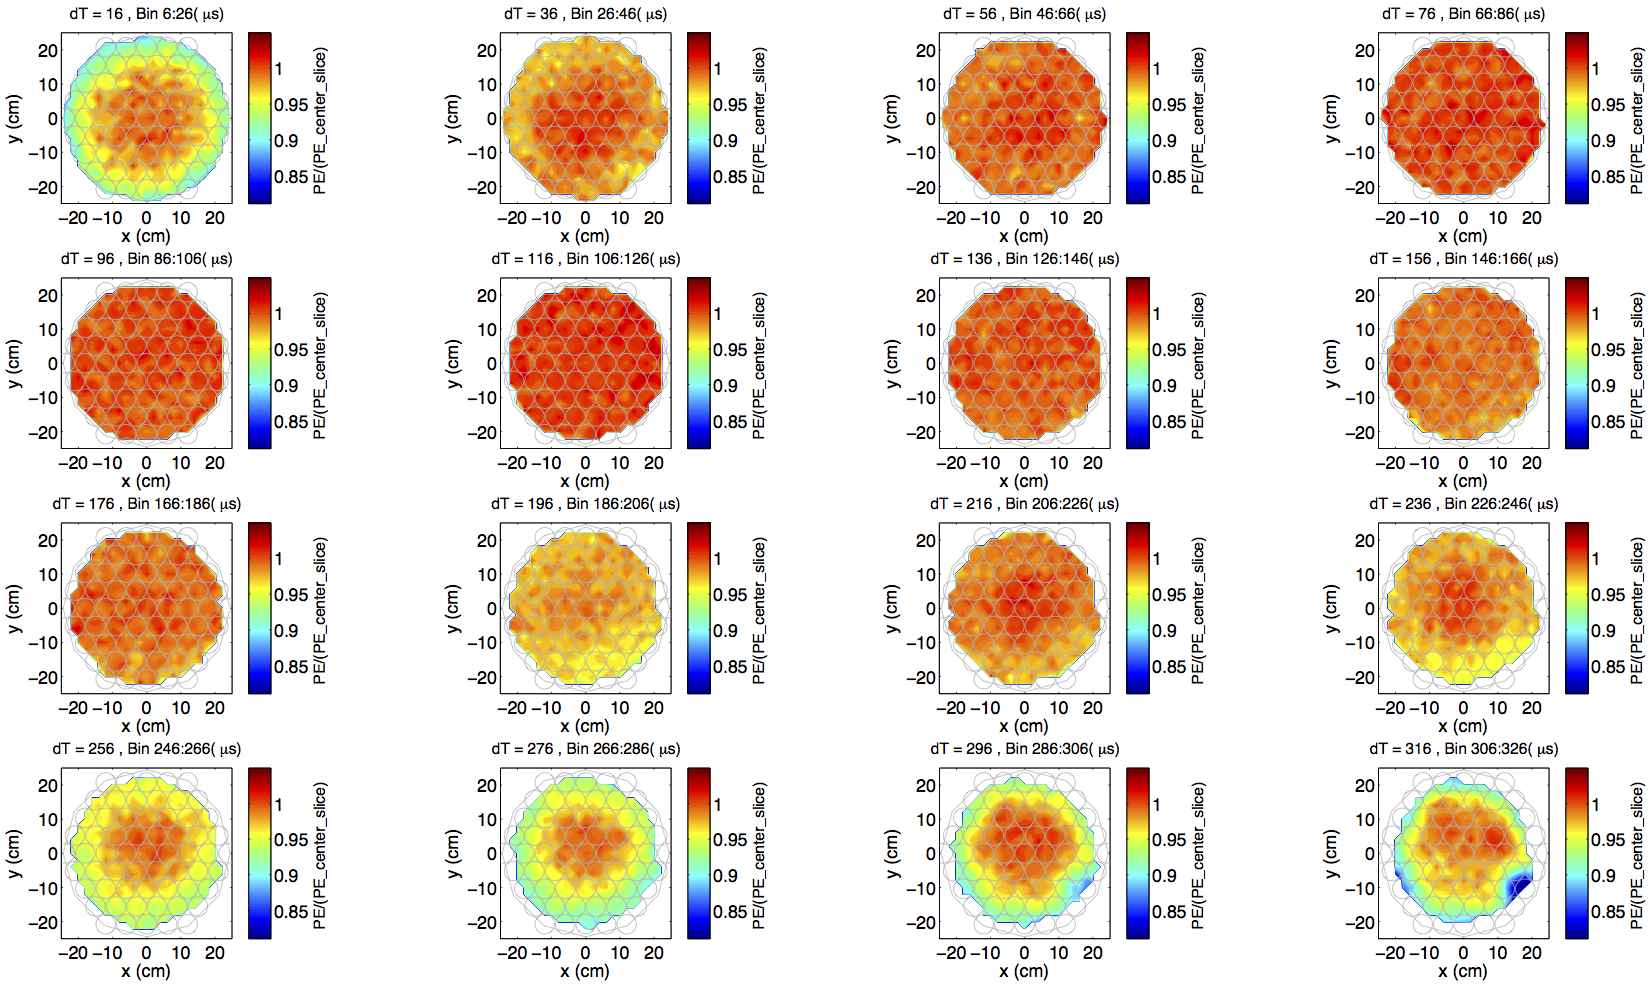
\includegraphics[width=230mm]{Chapter_XYZ_Corr/Thesis_Corr_Plots/S1_XYZ_Kr_norm_center_slice_crop.png}
\caption{S1 x,y,z response normalized to the center of each z slice. There are greater variations near the very top and bottom 4 z slices as the solid angle for light hitting the PMT arrays increases. For the central slices the x,y response is uniform due to increased scattering off the teflon panels. }
\label{fig:S1_XYZ_norm_center_slice}
\end{sidewaysfigure}
\renewcommand{\baselinestretch}{2}
\small\normalsize

\newpage

We define the position-dependent  (x,y,z) corrected S1 signal as $\rm S1{_c}$, normalized to the center of the detector (x=y=0 and z=160$\rm \mu s$) calculated as follows:
\begin{equation}
\rm S1_{c}= S1_{(x,z,y)}=S1 \cdot \mathcal{NF}_{S1}(x,y,z)
\label{eq:S1_XYZ}
\end{equation}

\noindent where $\rm S1_{c}$ is the x,y,z corrected S1 signal and $\rm \mathcal{NF}_{S1}(x,y,z)$ is the Normalization Factor of the sum of all PMTs for S1s and is a function of x,y,z. The interpolation of the inverse of $\rm \mathcal{NF}_{S1}(x,y,z)$ along the x,y grid in z slices is plotted in figure \ref{fig:S1_XYZ_norm_center}. The normalization factor is applied to the S1 data by using a spline interpolation of the x,y,z coordinate of each event relative to the bin centers $\rm \mathcal{NF}_{S1}(x,z,y)$. Figure \ref{fig:S1_XYZ_norm_center} shows the S1 response after correcting the data relative to the center of the detector. After applying the x,y,z correction the position-dependent variations decrease to less than 1\% in the inner radial 18 cm of the detector (the fiducial volume), with as much as 3\% variations near the top and bottom edges where the interpolation fails.

\renewcommand{\baselinestretch}{1}
\small\normalsize
\begin{sidewaysfigure}[p!]\centering
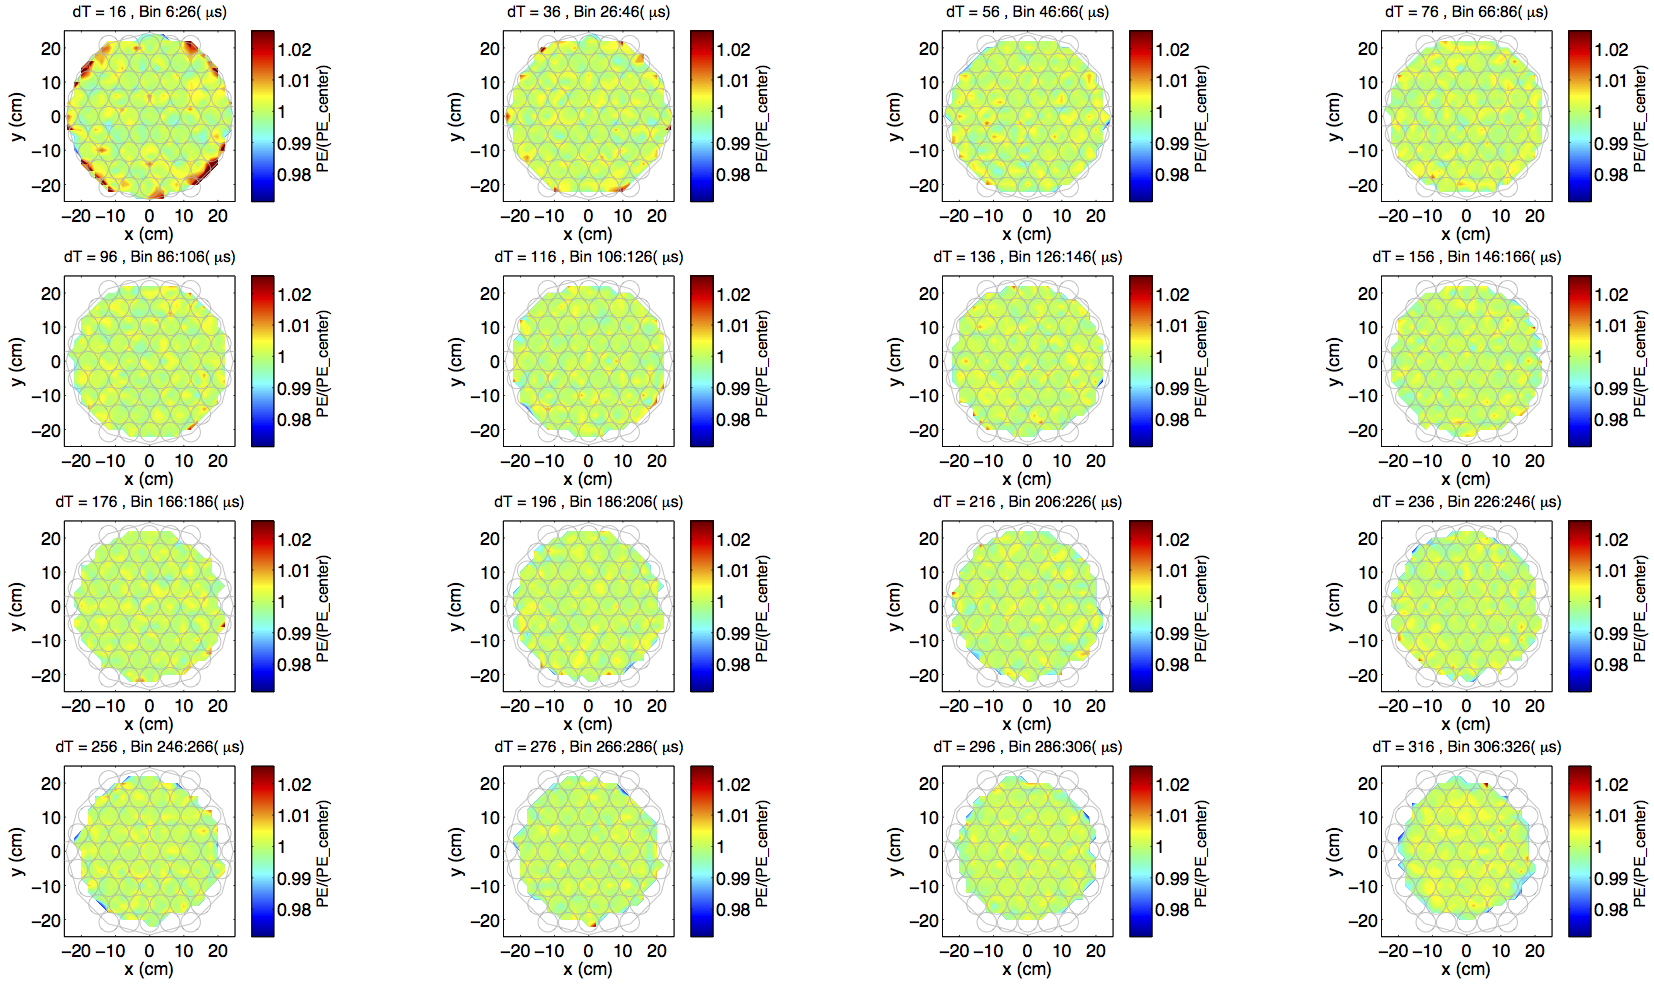
\includegraphics[width=220mm]{Chapter_XYZ_Corr/Thesis_Corr_Plots/S1_XYZ_Kr_FlatField_norm_center_crop.png}
\caption{S1 x,y,z response normalized to the center of the detector after the data has been corrected and normalized to the detector center. The remaining variations in the fiducial volume (r$<$18cm) is less than 1\%. Near the top and bottom edges the deviation increases to as much as 3\% due to the interpolation of the correction becoming poorly constrained.}
\label{fig:S1_XYZ_norm_center}
\end{sidewaysfigure}
\renewcommand{\baselinestretch}{2}
\small\normalsize


Figure \ref{fig:S1_res} shows the improvement in the S1 signal after applying the z and x,y,z correction. With z-only correction to S1 there is a fractional improvement in resolution of 31.5\%. The combined correction in z and the x,y plane provides an additional 2.0\% improvement in resolution over the z only correction.

\begin{figure}[h!]\centering
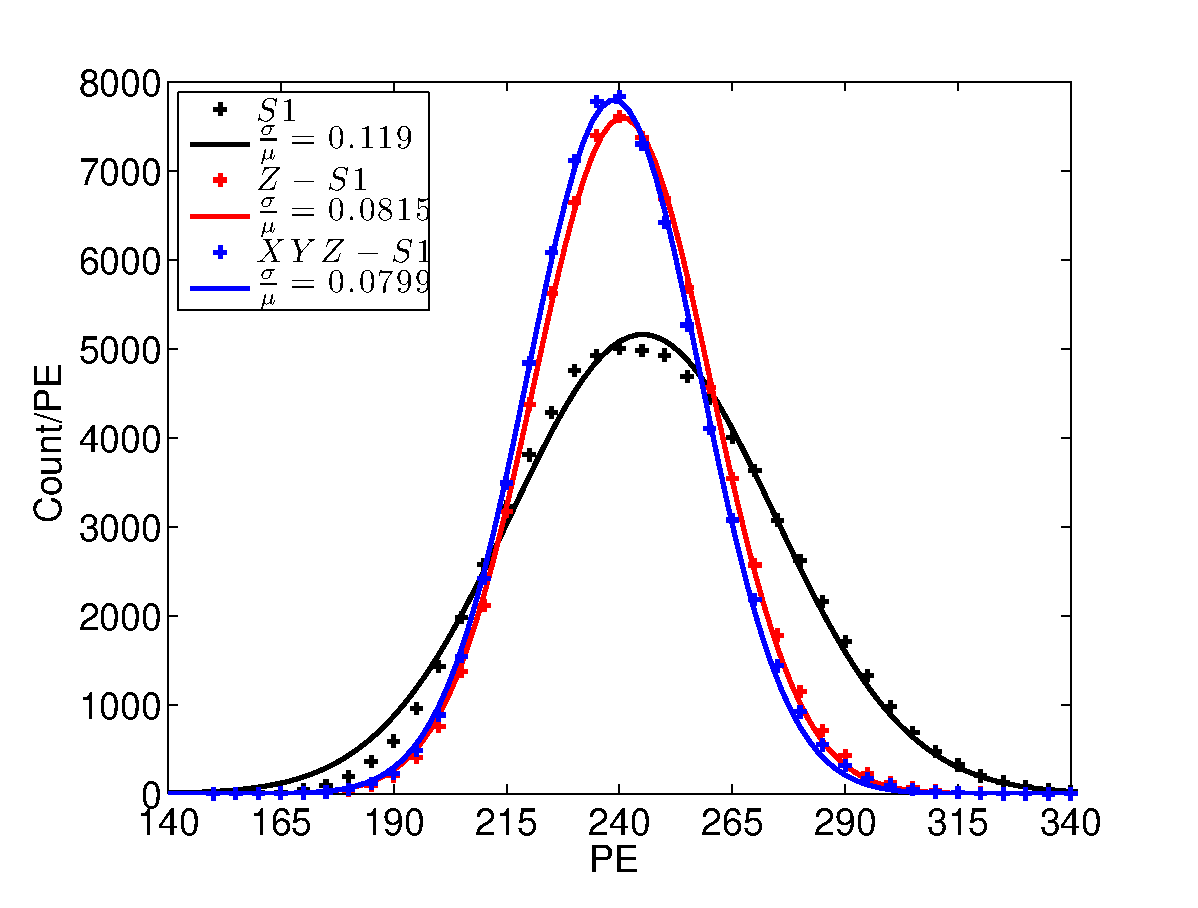
\includegraphics[width=100mm]{Chapter_XYZ_Corr/Thesis_Corr_Plots/S1_corr_res.eps}
\caption{Improvement of resolution in S1 after applying the z and x,y,z correction. Black: The uncorrected data. Red: The data with only z dependent correction. Blue: The data with full x,y,z dependent correction. The data shown was taken data on May 10, 2013 (lux10\_20130510\_T1250) and contains 700,000 \KrCal events.}
\label{fig:S1_res}
\end{figure}

\newpage

\section{Application of x,y,z Corrections to the Data}

As mentioned earlier, the purpose of the periodic \KrCal calibrations is to measure the position-dependent S1 and S2 corrections over the course of the 2013 science run. Before processing the WIMP search data the calibration sets were processed and a MYSQL table of electron lifetimes and corrections maps were populated for each calibration date. The electron lifetime applied to each WIMP search data set was a linear interpolation between calibration dates shown in figure \ref{fig:S2_EL_time}. The electron lifetimes measured for the science run are between 500 to 1000 $\rm \mu s$, or an attenuation length of 75 to 150 cm with a drift velocity of $\rm 1.51 mm/\mu s$. For the S2 x,y correction the nearest $\rm \mathcal{NF}_{S2}(x,y)$ entry in time was used. Combined these produced the corrected $\rm S2_c$ quantity to be used for the WIMP analysis. For the S1 x,y,z corrections, the nearest $\rm \mathcal{NF}_{S1}(x,y,z)$ entry is used to produce the corrected $\rm S1_c$ quantity via a spline interpolation in x,y,z. For both the S2-x,y and S1-x,y,z correction the time dependence is assumed to be negligible as these are geometric effects, whereas the electron lifetime varies with liquid purity each day.
The electron lifetime and the stability of the S1 correction over the course of the 2013 science run is shown in figure \ref{fig:S2_EL_time} and \ref{fig:S1_center_time}. While the electron lifetime needs frequent monitoring, the S1 x,y,z response is fixed over several months of running.
For the results discussed in the subsequent sections of the thesis we will only work with the x,y,z corrected S1 and $\rm S2_b$ pulses ( $\rm S1_c$ and $\rm S2{_b}_c$ respectively) .

\begin{figure}[h!]\centering
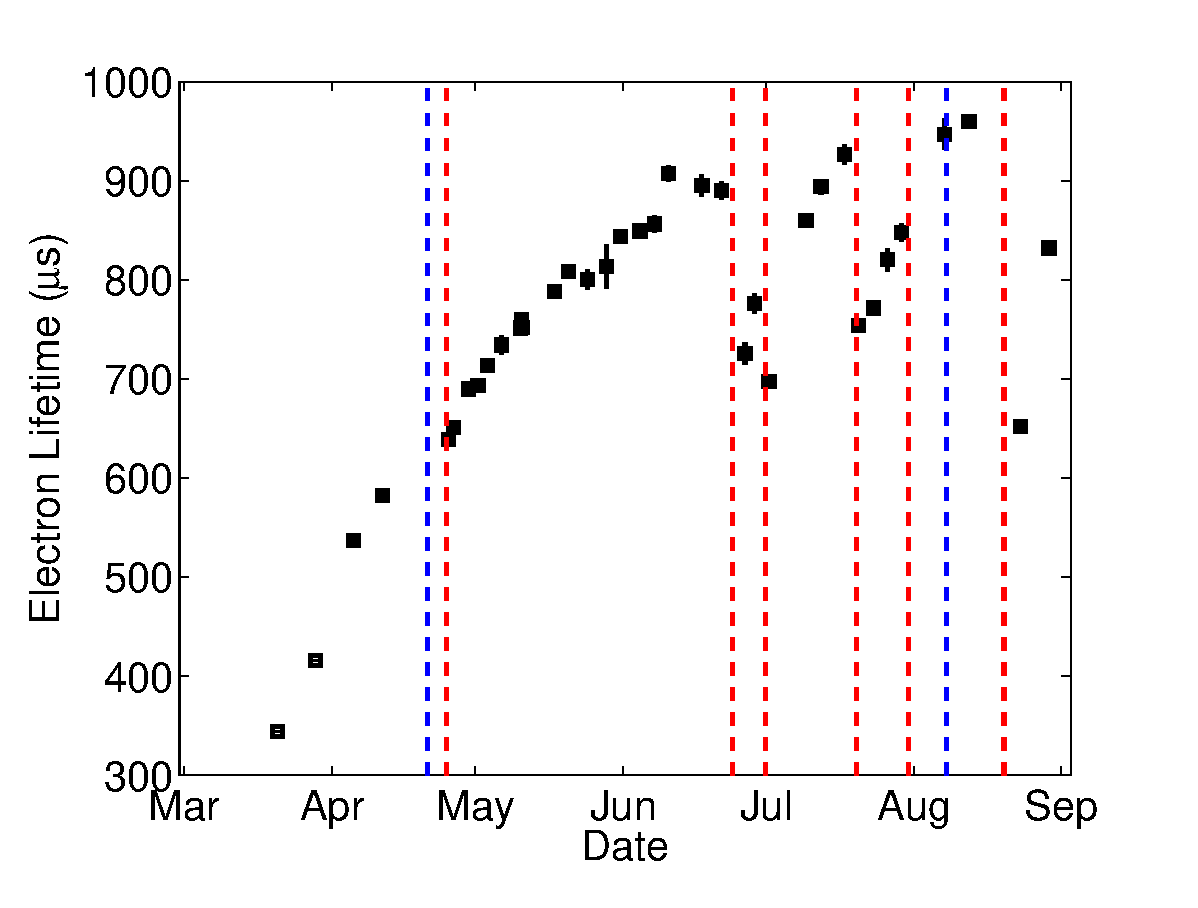
\includegraphics[width=100mm]{Chapter_XYZ_Corr/Thesis_Corr_Plots/lifetime_fig_3.eps}
\caption{Electron lifetime measured using \KrCal calibrations during the LUX science run in 2013. The blue dashed lines show the boundaries of the WIMP search from April 21 to Aug 8, 2013. The red dashed lines indicate circulation loss events.}
\label{fig:S2_EL_time}
\end{figure}

\begin{figure}[h!]\centering
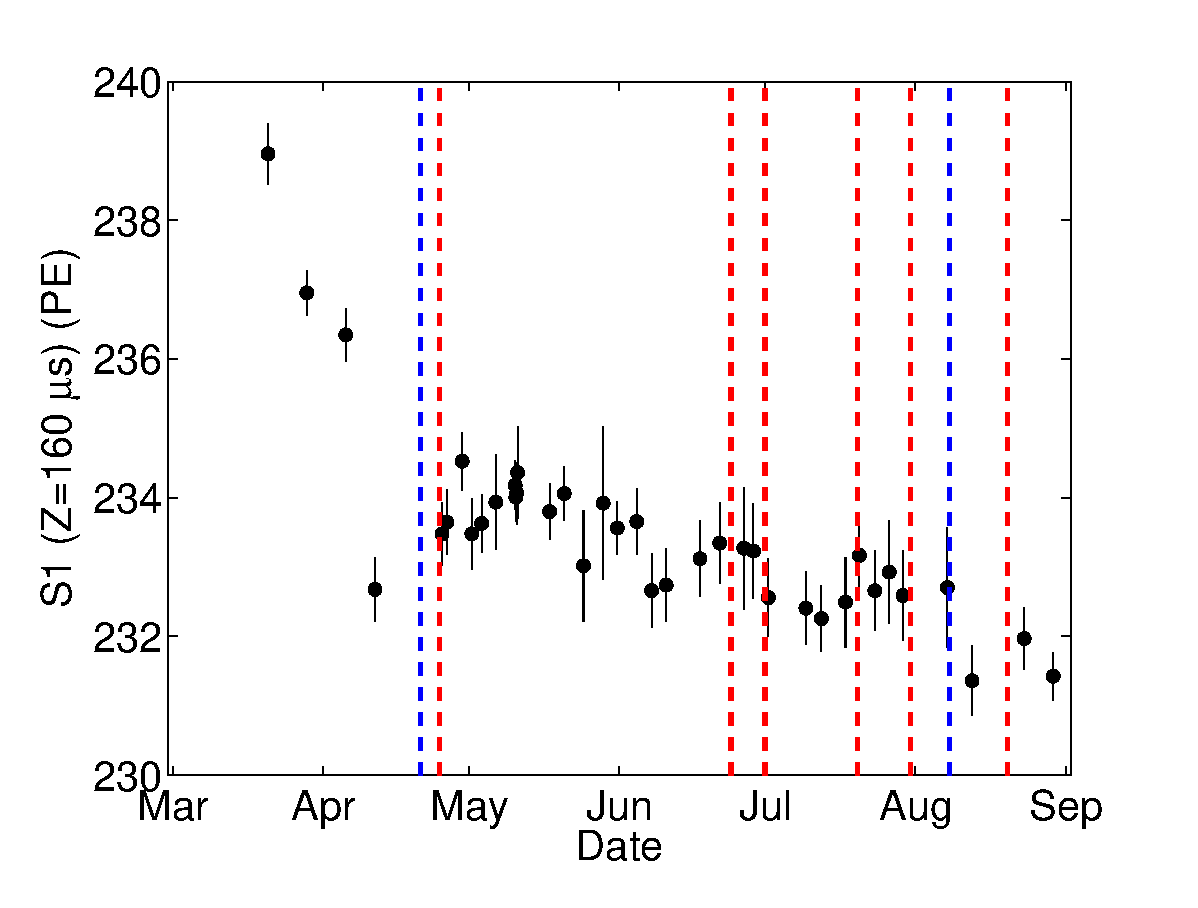
\includegraphics[width=100mm]{Chapter_XYZ_Corr/Thesis_Corr_Plots/s1_center_fig_3.eps}
\caption{Measured response of to light from \KrCal calibrations at the center of the LUX detector during of the LUX science run in 2013. The blue dashed lines show the boundaries of the WIMP search from April 21 to Aug 8, 2013. The red dashed lines indicate circulation loss events.}
\label{fig:S1_center_time}
\end{figure}


\renewcommand{\baselinestretch}{1}
\small\normalsize
\begin{table}[h!]
%\footnotesize
\begin{center}
\begin{tabular}{|c|c|}
\hline
\KrCal Calibration Set  &	 Number of \KrCal Events \\ 
lux10\_YYYYMMDDThhmm & 		\\ \hline
lux10\_20130320T1430	&	136,877	\\ \hline
lux10\_20130328T1437	&	444,622	\\ \hline
lux10\_20130405T1417	&	187,059	\\ \hline
lux10\_20130411T1524	&	99,724	\\ \hline
lux10\_20130425T1047	&	104,231	\\ \hline
lux10\_20130426T1019	&	92,024	\\ \hline
lux10\_20130429T1447	&	133,652	\\ \hline
lux10\_20130501T1508	&	91,465	\\ \hline
lux10\_20130503T1457	&	108,898	\\ \hline
lux10\_20130506T1328	&	45,678	\\ \hline
lux10\_20130510T1250	&	670,895	\\ \hline
lux10\_20130510T1607	&	499,743	\\ \hline
lux10\_20130510T2008	&	113,347	\\ \hline
lux10\_20130511T0014	&	44,372	\\ \hline
lux10\_20130517T1542	&	138,432	\\ \hline
lux10\_20130520T1504	&	216,709	\\ \hline
lux10\_20130524T1503	&	28,975	\\ \hline
lux10\_20130528T1546	&	11,569	\\ \hline
lux10\_20130531T1421	&	125,921	\\ \hline
lux10\_20130604T1421	&	110,219	\\ \hline
lux10\_20130607T1512	&	106,315	\\ \hline
lux10\_20130610T1518	&	116,349	\\ \hline
lux10\_20130617T1457	&	61,737	\\ \hline
lux10\_20130621T1533	&	78,707	\\ \hline
lux10\_20130626T1517	&	25,124	\\ \hline
lux10\_20130628T1444	&	44,134	\\ \hline
lux10\_20130701T1646	&	71,410	\\ \hline
lux10\_20130709T1009	&	106,230	\\ \hline
lux10\_20130712T1427	&	104,150	\\ \hline
lux10\_20130717T1424	&	66,801	\\ \hline
lux10\_20130720T1045	&	88,945	\\ \hline
lux10\_20130723T1452	&	88,626	\\ \hline
lux10\_20130726T1431	&	35,056	\\ \hline
lux10\_20130729T1004	&	59,906	\\ \hline
lux10\_20130807T1403	&	27,015	\\ \hline
lux10\_20130812T1546	&	113,560	\\ \hline
lux10\_20130823T0953	&	107,820	\\ \hline
lux10\_20130829T1005	&	479,676	\\ \hline
\end{tabular}
\caption{\KrCal sets used to calculating corrections for the 2013 LUX WIMP search \cite{LUX_PRL}.}
\label{table:Kr_Cal_Sets}
\end{center}
\end{table}
\renewcommand{\baselinestretch}{2}
\small\normalsize




